\documentclass[ignorenonframetext,10pt,aspectratio=169]{beamer}

\usepackage{umut}
\usepackage{umuttr}
\usepackage{usynsem}
\usepackage[utf8]{inputenc}
\usepackage{uling}
\usepackage{natbib,unatbib}
\usepackage{linguex}
         \renewcommand{\refdash}{}
\usepackage{ubeamer}
\usepackage{verbatim}
\usepackage{adjustbox}
\usepackage{fancyvrb}

\usepackage{tikz-qtree}
\usetikzlibrary{er,positioning}

\title{Agreement}
\author{\  \\  {\it Partly based on Koeneman \& Zeiljstra (2017)} \\ \vspace{20pt} Umut \"Ozge\\  }

\date{COGS 532: Theoretical Linguistics\\ METU, Informatics}

\begin{document}

\begin{frame}\frametitle{}
\thispagestyle{empty}
\maketitle
\end{frame}

\begin{frame}[t,plain]{Interpretable versus uninterpretable features}

		\ex.\a.  *John walk.
		\b. *I walks.
		\b. *They walks.

\end{frame}

\begin{frame}[t,plain]{}
		\ex. John loves Mary.

\begin{center}
\adjustbox{valign=t}{
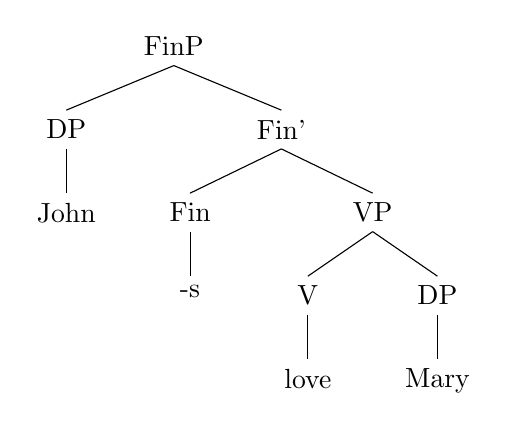
\begin{tikzpicture}
\tikzset{level distance=30pt, sibling distance=20pt}
\tikzset{every tree node/.style={align=center,anchor=north}}
				\Tree
				[.{FinP}
					[.{DP} John ]
					[.{Fin'} 
						[.{Fin} -s ]
							[.{VP}
								[.{V} love ] 
								[.{DP} Mary ] 
							]
					]
				]
\end{tikzpicture}}
\end{center}

\end{frame}

\begin{frame}[t,plain,label=jlm]{}

		\ex. John loves Mary.

\begin{center}
\adjustbox{valign=t}{
\begin{tikzpicture}
\tikzset{level distance=30pt, sibling distance=20pt}
\tikzset{every tree node/.style={align=center,anchor=north}}
				\Tree
				[.{FinP}
					[.{DP} John\\{\begin{avm} \[cat  & n \\ det & + \\ $\phi$  & 3, sg\] \end{avm}} ]
					[.{Fin'} 
						[.{Fin} -s\\{\begin{avm} \[cat  & fin \\ finite  & + \\ $\phi^{(u)}$  & 3, sg\] \end{avm}} ]
							[.{VP}
								[.{V} love ] 
								[.{DP} Mary\\{\begin{avm} \[cat  & n \\ det & + \\ $\phi$  & 3, sg\] \end{avm}} ] 
							]
					]
				]
\end{tikzpicture}}
\end{center}

\end{frame}

\begin{frame}[t,plain]{Agreement (to be revised)}

		\vspace{40pt}

In a tree $\Gamma$, if there is a node $\alpha$ with \setavm{\[F$^{(u)}$\]}, then there needs to be another node $\beta$ with \setavm{\[F\]}, such that there are no maximal projection nodes that include $\alpha$ without including $\beta$ or vice versa.
	

\end{frame}

\againframe{jlm}

\begin{frame}[t,plain]{}

		\ex. *I loves Mary.

\begin{center}
\adjustbox{valign=t}{
\begin{tikzpicture}
\tikzset{level distance=30pt, sibling distance=20pt}
\tikzset{every tree node/.style={align=center,anchor=north}}
				\Tree
				[.{FinP}
					[.{DP} I\\{\begin{avm} \[cat  & n \\ det & + \\ $\phi$  & 1, sg\] \end{avm}} ]
					[.{Fin'} 
						[.{Fin} -s\\{\begin{avm} \[cat  & fin \\ finite  & + \\ $\phi^{(u)}$  & 3, sg\] \end{avm}} ]
							[.{VP}
								[.{V} love ] 
								[.{DP} Mary\\{\begin{avm} \[cat  & n \\ det & + \\ $\phi$  & 3, sg\] \end{avm}} ] 
							]
					]
				]
\end{tikzpicture}}
\end{center}
\end{frame}

\begin{frame}[t,plain]{}

\end{frame}


\begin{frame}[t,plain]{}
\begin{center}
\begin{tikzpicture}
\tikzset{level distance=30pt, sibling distance=20pt}
\tikzset{every tree node/.style={align=center,anchor=north}}


\end{tikzpicture}
\end{center}
\end{frame}

\begin{frame}[t,plain]{}


\end{frame}

\begin{frame}[t,plain]{}

\end{frame}

\begin{frame}[t,plain]{}

\end{frame}

\begin{frame}[t,plain]{}

\end{frame}

\begin{frame}[t,plain]{}

\end{frame}

\end{document}
